% -*- Mode:TeX -*-

%% The documentclass options along with the pagestyle can be used to generate
%% a technical report, a draft copy, or a regular thesis.  You may need to
%% re-specify the pagestyle after you \include  cover.tex.  For more
%% information, see the first few lines of sk-thesis.cls. 

% DRAFT MODE uses simpler front page, without dedication, acknowledgements, uses a footer sying draft.
%\documentclass[12pt,a4paper,vi,twoside,leftblank]{sk-thesis}
%\documentclass[12pt,a4paper,vi,draft]{sk-thesis}
\documentclass[12pt,a4paper,vi]{sk-thesis}
\usepackage[utf8]{inputenc}
\usepackage{geometry}
\geometry{a4paper, right=30mm, bottom=30mm, left=30mm, top=30mm}

\usepackage{ifdraft}
\usepackage{graphicx}
\setkeys{Gin}{draft=false} % disable hiding graphics in draft mode
\usepackage[table]{xcolor}
\usepackage{multicol, multirow}
\usepackage{amsmath, amssymb}
\usepackage{cmap}
\usepackage[T1]{fontenc}
\setlength {\marginparwidth }{2.5cm} 
\usepackage[obeyDraft]{todonotes}
\usepackage{booktabs, siunitx}
\usepackage[breaklinks=true]{hyperref}
\usepackage{natbib, breakcites}
\usepackage{bibentry}
\usepackage{doi}
\definecolor{navyblue}{rgb}{0.0, 0.0, 0.5}
%\definecolor{royalblue}{rgb}{0.06, 0.11, 0.42}
\hypersetup{
  final,
  colorlinks=true,
  urlcolor=navyblue,
  citecolor=navyblue,
  linkcolor=navyblue
}
\usepackage{cleveref}
\crefformat{footnote}{#2\footnotemark[#1]#3}
%\usepackage{catoptions}
\makeatletter
%\def\figureautorefname{figure}
%\def\tableautorefname{table}
\def\Autoref#1{%
  \begingroup
  \edef\reserved@a{\cpttrimspaces{#1}}%
  \ifcsndefTF{r@#1}{%
    \xaftercsname{\expandafter\testreftype\@fourthoffive}
      {r@\reserved@a}.\\{#1}%
  }{%
    \ref{#1}%
  }%
  \endgroup
}
\def\testreftype#1.#2\\#3{%
  \ifcsndefTF{#1autorefname}{%
    \def\reserved@a##1##2\@nil{%
      \uppercase{\def\ref@name{##1}}%
      \csn@edef{#1autorefname}{\ref@name##2}%
      \autoref{#3}%
    }%
    \reserved@a#1\@nil
  }{%
    \autoref{#3}%
  }%
}
\makeatother
\usepackage{textcomp}
\usepackage{fancyhdr}
\newcommand{\changefont}{%
    \fontsize{10}{10}\selectfont
}
\fancyhf{}
%\fancyhead[LE]{\slshape \rightmark} %section
%\fancyhead[RE]{}
%\fancyhead[RO]{\slshape \leftmark} % chapter
%\fancyhead[LO]{}
\fancyhead[LE,RO]{\changefont \slshape \nouppercase{\rightmark}} %section
\fancyhead[RE,LO]{\changefont \slshape \nouppercase{\leftmark}} %chapter
\fancyfoot[C]{\thepage} %footer
\usepackage{datetime}
\usepackage[automake,toc]{glossaries}
\glsenablehyper
\makeglossaries
%\usepackage{comment}
\usepackage{subcaption}
\usepackage{tabularx, lscape, rotating}
\usepackage[most]{tcolorbox}
\newtcolorbox{myframe}[1][]{
  enhanced,
  top=12pt,bottom=12pt,left=16pt,right=16pt,
  arc=0pt,
  outer arc=0pt,
  colback=white,
  boxrule=1pt,
  #1
}

%%%%%%%%%%%% EPIGRAPH
\usepackage{epigraph}
%\setlength{\beforeepigraphskip}{1.0\baselineskip}
\setlength{\epigraphrule}{0pt}
\setlength{\epigraphwidth}{.4\textwidth}
%\setlength{\afterepigraphskip}{.25\baselineskip}
\renewcommand{\textflush}{flushepinormal}

\ifdraft{
    %% LIMIT CHAPTERS
    \includeonly{
        prelude,
        contents,
        chapters/introduction,
        chapters/background,
        chapters/thesis-objectives,
        chapters/conclusion,
        glossary,
        bibliography,
        chapters/appendix-a
    }
} { }

\begin{document}

\ifdraft{
    %%%%%%%%%%% HEADERS AND FOOTERS
    \fancypagestyle{plain}{%
      \fancyhf{}%
      \renewcommand{\headrulewidth}{0pt}% Line at the header invisible
      \fancyfoot[L]{\changefont PhD Thesis - Student Name} % DRAFT ONLY
      \fancyfoot[C]{\thepage}% \changefont 
      \fancyfoot[R]{\changefont \textbf{DRAFT} \today} % DRAFT ONLY
    }
    \fancyfoot[L]{\changefont PhD Thesis - Student Name} % DRAFT ONLY
    \fancyfoot[R]{\changefont \textbf{DRAFT} \today} % DRAFT ONLY
    \pagestyle{fancy}
    
    %% SIMPLE TITLE PAGE
    \chapter*{Thesis Title}

\begin{center}
\Large{
\textsc{PhD Thesis (Final Draft) \\ Student Name \\ }
}

\today\ \currenttime
\end{center}

\clearpage

\section*{Abstract}
In short this is the content of my work...

\section*{Publications}
\subsection*{Main author}
\nobibliography*

\begin{enumerate}
    \item \bibentry{Skoltech2017}
\end{enumerate}

\subsection*{Co-author}

\begin{enumerate}
    \item \bibentry{Skoltech2017}
\end{enumerate}

\listoftodos
\clearpage
}{
    %% FULL TITLE PAGE
    % -*-latex-*-
% NOTE:
% These templates make an effort to conform to the Skoltech Thesis specifications,
% however the specifications can change.  We recommend that you verify the
% layout of your title page with your thesis advisor and the Education department 
% before printing your final copy.
\title{Thesis Template Skoltech}

\author{Student Name}
% If you wish to list your previous degrees on the cover page, use the 
% previous degrees command:
%       \prevdegrees{MSc, University of Salzburg (2007)}
% You can use the \\ command to list multiple previous degrees
%       \prevdegrees{B.S., University of California (1978) \\
%                    S.M., Massachusetts Institute of Technology (1981)}
\department{Skoltech Center of Research, Entrepreneurship and Innovation}

\degree{Doctoral Program in Engineering Systems}

\degreemonth{November}
\degreeyear{2019}
\thesisdate{November 2019}

%% By default, the thesis will be copyrighted to MIT.  If you need to copyright
%% the thesis to yourself, just specify the `vi' documentclass option.  If for
%% some reason you want to exactly specify the copyright notice text, you can
%% use the \copyrightnoticetext command.  
%\copyrightnoticetext{\copyright \@author \@degreeyear}

% If there is more than one supervisor, use the \supervisor command
% once for each.
\supervisor{Edward Crawley}{Founding President, Professor}

% This is the department committee chairman, not the thesis committee
% chairman.  You should replace this with your Department's Committee
% Chairman.
%\chairman{Name}{Title}

% Make the titlepage based on the above information.  If you need
% something special and can't use the standard form, you can specify
% the exact text of the titlepage yourself.  Put it in a titlepage
% environment and leave blank lines where you want vertical space.
% The spaces will be adjusted to fill the entire page.  The dotted
% lines for the signatures are made with the \signature command.
\maketitle

% The abstractpage environment sets up everything on the page except
% the text itself.  The title and other header material are put at the
% top of the page, and the supervisors are listed at the bottom.  A
% new page is begun both before and after.  Of course, an abstract may
% be more than one page itself.  If you need more control over the
% format of the page, you can use the abstract environment, which puts
% the word "Abstract" at the beginning and single spaces its text.

%% You can either \input (*not* \include) your abstract file, or you can put
%% the text of the abstract directly between the \begin{abstractpage} and
%% \end{abstractpage} commands.

% First copy: start a new page, and save the page number.
\cleardoublepage
% Uncomment the next line if you do NOT want a page number on your
% abstract and acknowledgments pages.
% \pagestyle{empty}
\setcounter{savepage}{\thepage}
\begin{abstractpage}
In short this is the content of my work...
\end{abstractpage}


\clearpage
\section*{Publications}
\subsection*{Main author}
\nobibliography*

\begin{enumerate}
    \item \bibentry{Skoltech2017}
\end{enumerate}

\subsection*{Co-author}

\begin{enumerate}
    \item \bibentry{Skoltech2017}
\end{enumerate}

\cleardoublepage

\begin{dedication}
Dedicated to my parents.
\end{dedication}

\section*{Acknowledgments}

Let me thank to all my supporters ...

    
    %%%%%%%%%%% HEADERS AND FOOTERS
    \fancypagestyle{plain}{%
      \fancyhf{}%
      \renewcommand{\headrulewidth}{0pt}% Line at the header invisible
      \fancyfoot[C]{\thepage}%
    }
    \pagestyle{fancy}
}
  % -*- Mode:TeX -*-
%% This file simply contains the commands that actually generate the table of
%% contents and lists of figures and tables.  You can omit any or all of
%% these files by simply taking out the appropriate command.  For more
%% information on these files, see appendix C.3.3 of the LaTeX manual.

\begin{singlespace}
    \tableofcontents
\end{singlespace}
\newpage
%\ifdraft{
%}{
\begin{singlespace}
    \listoffigures
\end{singlespace}
\newpage
\begin{singlespace}
    \listoftables
\end{singlespace}
%}
\chapter{Introduction}

Let me introduce to the topic of my PhD 

Design, manufacturing and developing software for an omnidirectional agricultural robot.

The solution comes in the form of a 4-wheeled robot 

The proposed solution comprises the following modules:

\begin{itemize}
    \item chassis
    \item wheel base
    \item electrics
    \item sensing, computation and communication
    \item software
\end{itemize}

The software could in turn be broken down into the following:

\begin{itemize}
    \item data transport
    \item localization
    \item target CV problem
    \item logging and data representation
    \item path planning
    \item user interface
\end{itemize}

Let us describe each of the elements of the system in detail.

chassis

The main structural elements of the robot's frame are manufactured from the aluminum profile (tube with rectangular cross-section).
They were designed to withstand the loads that exceed the normal ones with a huge margin.
The rigidity is assured by a rectangular section of a composite material (alucobond) that separates the inner volume of the robot into two.
The tubes were connected by flat milled aluminum elements.
The assembly was performed using bolts and nuts, as well as rivets and bits of welding.
The total weight of the chassis if N \si{kg}.

wheel base

The wheels were designed to work in pairs: each omnidirectional wheel is mechanically coupled with a rail wheel

electrics



sensing, computation and communication



software



data transport



localization



target CV problem



logging and data representation



path planning



user interface



\todo[inline]{TODO: complete chapter}

\section{Thesis Structure}
The diagram in \ref{fig:thesis-structure} illustrates the flow of information through the structure of the thesis.



\begin{figure}[htb!]
\centering 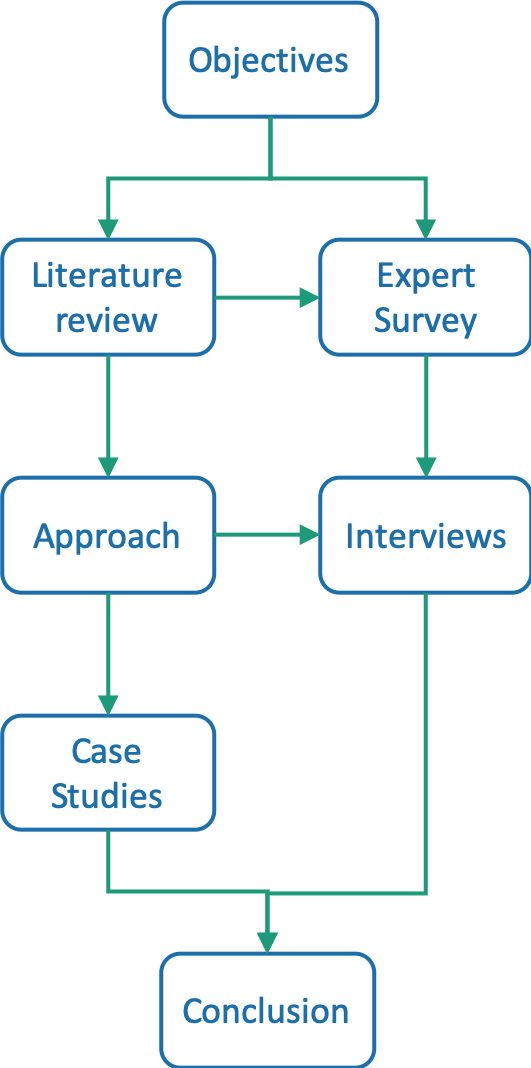
\includegraphics[width=0.5\textwidth]{graphics/thesis-structure}
\caption{Thesis structure}
\label{fig:thesis-structure}
\end{figure}

\begin{description}
    \item[\ref{cap:background} - Background]
Here's the literature review.

    \item[\ref{cap:thesis_objectives} - Thesis Objectives]
We define the objectives of our work.

...

    \item[\ref{cap:conclusion} - Conclusion]
In the last chapter, we discuss our results obtained ...

\end{description}


\chapter{Background}
\label{cap:background}
\epigraphhead[50]{%
    \epigraph{"if I have seen further it is by standing on the shoulders of Giants."}{Isaac Newton, 1675}
}

Here is a comprehensive review of the literature related to the topic of this work.

We inspired our work from \citet{Chakrabarti2014}.
\acrshort{sysml} is the reference in this field \citep{ObjectManagementGroup2015}
The tools keep evolving \citep{Skoltech2017}.

\todo[inline]{TODO: complete chapter}
\chapter{Thesis Objectives}
\label{cap:thesis_objectives}

In this chapter we define the goals and derive the specific questions to be addressed in our research.

\chapter{Conclusion}
\label{cap:conclusion}

\epigraphhead[50]{%
    \epigraph{"If you optimize everything, you will always be unhappy."}{Donald Knuth}
}

In this last chapter, we discuss the results, the limitations of our work, and provide an outlook on future work. 



\newacronym{sk}{SK}{Skolkovo Institute of Science and Technology}
\newacronym{sysml}{SysML}{Systems Modeling Language}

\begin{singlespace}
\printglossary
\end{singlespace}

\phantomsection 
\addcontentsline{toc}{chapter}{Bibliography} 
%% This defines the bibliography file (main.bib) and the bibliography style.
%% If you want to create a bibliography file by hand, change the contents of
%% this file to a `thebibliography' environment.  For more information 
%% see section 4.3 of the LaTeX manual.
\begin{singlespace}
\bibliographystyle{plainnat}
\bibliography{references}
\end{singlespace}


\appendix
\chapter{Additional Resources}
\label{sec:additional-resources}

\Autoref{tab:comparison_x_and_y} contains some additional material.

\setlength{\tabcolsep}{0.5em} % for the horizontal padding
\renewcommand{\arraystretch}{2} % for the vertical padding
\begin{table}[ht!]
  \centering
  \begin{tabularx}{0.9\textwidth}{|p{8em}|p{6em}p{6em}X|}
    \hline
    \textbf{Feature}     & \textbf{Method X}      & \textbf{Method Y}                           & \textbf{References}                      \\
    \hline
    \rowcolor[HTML]{EFEFEF}
    Speed                     &  medium     &  slow          &       Skoltech2017             \\
    \hline
    Cost                        & less            & more          &                                  \\
    \hline
    \rowcolor[HTML]{EFEFEF}
    Error                      &        2           &                   3                   &                                         \\
    \hline
  \end{tabularx}
    \caption{Comparison of X and Y}
    \label{tab:comparison_x_and_y}%
\end{table}

\end{document}

